% !TEX program = xelatex
\documentclass[12pt,a4paper]{article}
\usepackage{polyglossia}
\setmainlanguage{arabic}
\setotherlanguage{english}
\usepackage{amsmath,amssymb}
\usepackage{graphicx}
\usepackage{booktabs}
\usepackage{hyperref}
\usepackage{fontspec}
\setmainfont{Arial}
\newfontfamily\arabicfont[Script=Arabic]{Arial}
\usepackage[margin=2.5cm]{geometry}

\usepackage{amsthm}
\newcommand{\R}{\mathbb{R}}
\newtheoremstyle{arabicremark}{}{}{}{}{\bfseries}{.}{ }{}
\theoremstyle{arabicremark}
\newtheorem{remark}{ملاحظة}

\title{\textbf{تقدير الأداء المقيّد بالرتبة عبر تحليل بورير-مونتيرو}}
\author{غيداء نجيب خضور \and جميل ابراهيم جوني}
\date{}

\begin{document}
\maketitle

\begin{abstract}
ندرس مشكلة تقدير الأداء المقيّدة بالرتبة (PEP) لحساب حدود الأسوأ أداء لطرق التحسين من الجهود الأولى. تقوم صيغة PEP القياسية بتفريغ قيد الرتبة على مصفوفة غرام، مما قد يُحلّف الأداء. نعيد صياغة مشكلة PEP المقيّدة بالرتبة كمسألة تحسين مقيدة ذات تربيعات (QCQP) عبر تحليل بورير-مونتيرو $G = VV^\top$ مع $d$ عمودًا، مما يُنتج مشكلة غير محدبة منخفضة الأبعاد قابلة للحل بمحليات جاهزة. عند التحقق من صلاحية طريقة التدرج بخطوة $h=1/L$، نستخرج حدود دروري-تبول إلى دقة الآلة الحاسبة. تؤكد تجاربنا أن قيد الرتبة غير فعّال للتدرج التصاعدي، مما يؤكد أن ارتخاء SDP متسق لهذه الطريقة عبر جميع الأبعاد المختبرة.
\end{abstract}

\section{المقدمة}

مُشكّلة تقدير الأداء (PEP)، التي قدّمها دروري وتيبول، توفر إطارًا منهجيًا لحساب ضمانات الأسوأ أداء لطرق التحسين من الجهود الأولى على فئة الدوال $L$-منمّمة ومحدبة.

تُصاغ PEP عادةً كبرنامج شبه محدبي (SDP) فوق مصفوفة غرام:
\[
G = \begin{pmatrix} X & G_{xg} \\ G_{xg}^\top & G_{gg} \end{pmatrix},
\]
حيث $X_{ij} = \langle x_i - x_*, x_j - x_*\rangle$، $(G_{xg})_{ij} = \langle x_i - x_*, g_j\rangle$، و$(G_{gg})_{ij} = \langle g_i, g_j\rangle$. يقوم SDP بتفريغ قيد $\operatorname{rank}(G) \leq 2d$، مما قد يُحدث تخفيفًا للأداء عندما يكون $d$ صغيرًا مقارنةً بـ$N$.

أثبت تايلور وهيندريكس وغلينور أن قيد الرتبة غير فعّال عندما $d \geq N+2$، لكنهم تركوا الحالة $d < N+2$ كمسألة مفتوحة. نملأ هذه الفجوة عددانيًا عبر إعادة صياغة PEP المقيّدة بالرتبة باستخدام تحليل بورير-مونتيرو.

\section{صيغة المشكلة}

\subsection{PEP القياسية}

لأول طريقة تُولّد السلاسل $x_0, x_1, \ldots, x_N$ مع التدرجات $g_0, g_1, \ldots, g_N$، تكون PEP للدوال $L$-منمّمة ومحدبة:
\begin{align}
\max_{G \succeq 0, \{f_k\}} \quad & f_N - f_* \\
\text{s.t.} \quad & G_{x_0 x_0} \leq R^2 \quad \text{(IC)} \\
& f_i - f_* - \langle g_i, x_i - x_*\rangle + \frac{1}{2L}\|g_i\|^2 \leq 0 \quad \text{(OPT)} \\
& f_i - f_j - \langle g_j, x_i - x_j\rangle + \frac{1}{2L}\|g_i - g_j\|^2 \leq 0 \quad \text{(INT)} \\
& \operatorname{rank}(G) \leq 2d
\end{align}
حيث $R = \|x_0 - x_*\|$ و$f_* = 0$ (تطبيع).

\subsection{إعادة الصياغة عبر بورير-مونتيرو}

نضع $f_* = 0$ و$x_* = 0$. نعرّف $v_{s_i} = x_i - x_*$ و$v_{y_i} = g_i / L$. يُلبّى قيد الرتبة $\operatorname{rank}(G) \leq d$ تلقائيًا عبر التحليل $G = VV^\top$ حيث:
\[
V = \begin{pmatrix} V_s \\ L \cdot V_y \end{pmatrix}, \quad V_s = (v_{s_0}, \ldots, v_{s_N})^\top \in \R^{(N+1)\times d}, \quad V_y = (v_{y_0}, \ldots, v_{y_N})^\top \in \R^{(N+1)\times d}.
\]

بعد التطبيع وإزالة خطوة التدرج $v_{s_{i+1}} = v_{s_i} - h L v_{y_i}$ (مع $h = 1/L$)، تصبح QCQP:
\begin{align}
\max_{V_s, V_y, f} \quad & f_N \\
\text{s.t.} \quad & \|v_{s_0}\|^2 \leq R^2 \\
& f_i \geq \frac{L}{2}\|v_{y_i}\|^2 \quad \text{(الحد الأدنى OPT)} \\
& f_i \leq L\langle v_{y_i}, v_{s_i}\rangle - \frac{L}{2}\|v_{y_i}\|^2 \quad \text{(الحد الأعلى OPT)} \\
& f_i - f_j - L\langle v_{y_j}, v_{s_i} - v_{s_j}\rangle - \frac{L}{2}\|v_{y_i} - v_{y_j}\|^2 \geq 0 \quad \text{(INT)}
\end{align}

\begin{remark}
قيد الحد الأعلى OPT ينشأ من التداخل عند النقطة المثلى وهو ضروري للبرهانية. بدونه، $f_N \to \infty$ ممكن.
\end{remark}

\section{الطريقة العددية}

نحلّ QCQP عبر التخسيس مع L-BFGS-B:
\[
\min_\theta \; -f_N + \mu \sum_{\text{القيود}} [\text{الإخلال}]^2_+
\]
باستخدام جدول تخسيس متسلسل $\mu \in \{1, 10, 10^2, \ldots, 10^6\}$ مع البدء الدافئ. تُحلّ كل مشكلة من تهيئة عشوائية متعددة (15-30 إعادة بدء).

\section{التحقق والنتائج}

\subsection{فحوصات السلمية}

نتحقق من حدود دروري-تبول $f_N \leq \frac{1}{4N+2}$ للتدرج التصاعدي مع $h = 1/L$:
\begin{itemize}
\item $N=1$، $d=1$: يُعطي المحلل $0.16666705$ مقابل دروري $1/6 = 0.166667$. الفجوة $< 10^{-6}$.
\item $N=3$، $d=5$: يُعطي المحلل $0.07142784$ مقابل دروري $1/14 = 0.071429$. الفجوة $< 10^{-6}$.
\item $N=5$، $d=6$: يُعطي المحلل $0.04545268$ مقابل دروري $1/22 = 0.045455$. الفجوة $< 10^{-6}$.
\end{itemize}

\subsection{حساسية الرتبة}

الجدول يُظهر حد الرتبة المقيّدة $f_N$ لكل $(N, d)$ مع $1 \leq N \leq 6$ و$1 \leq d \leq N+1$.

\begin{table}[h]
\centering
\caption{حد PEP المقيّد بالرتبة $f_N$ للتدرج التصاعدي ($h=1/L$، $L=1$، $R=1$).}
\label{tab:heatmap}
\begin{tabular}{c|cccccc|cc}
\toprule
$N$ & $d{=}1$ & $d{=}2$ & $d{=}3$ & $d{=}4$ & $d{=}5$ & $d{=}6$ & دروري & OGM$_{\mathrm{ref}}$ \\
\midrule
1 & 0.166667 & 0.166667 & --- & --- & --- & --- & 0.166667 & 0.125000 \\
2 & 0.100000 & 0.100000 & 0.100000 & --- & --- & --- & 0.100000 & 0.061894 \\
3 & 0.071429 & 0.071428 & 0.071428 & 0.071428 & --- & --- & 0.071429 & 0.037692 \\
4 & 0.055556 & 0.055554 & 0.055554 & 0.055554 & 0.055554 & --- & 0.055556 & 0.025584 \\
5 & 0.045455 & 0.045452 & 0.045453 & 0.045452 & 0.045453 & 0.045453 & 0.045455 & 0.018588 \\
6 & 0.038462 & 0.038459 & 0.038459 & 0.038459 & 0.038459 & 0.038459 & 0.038462 & --- \\
\bottomrule
\end{tabular}
\end{table}

\begin{figure}[h]
\centering
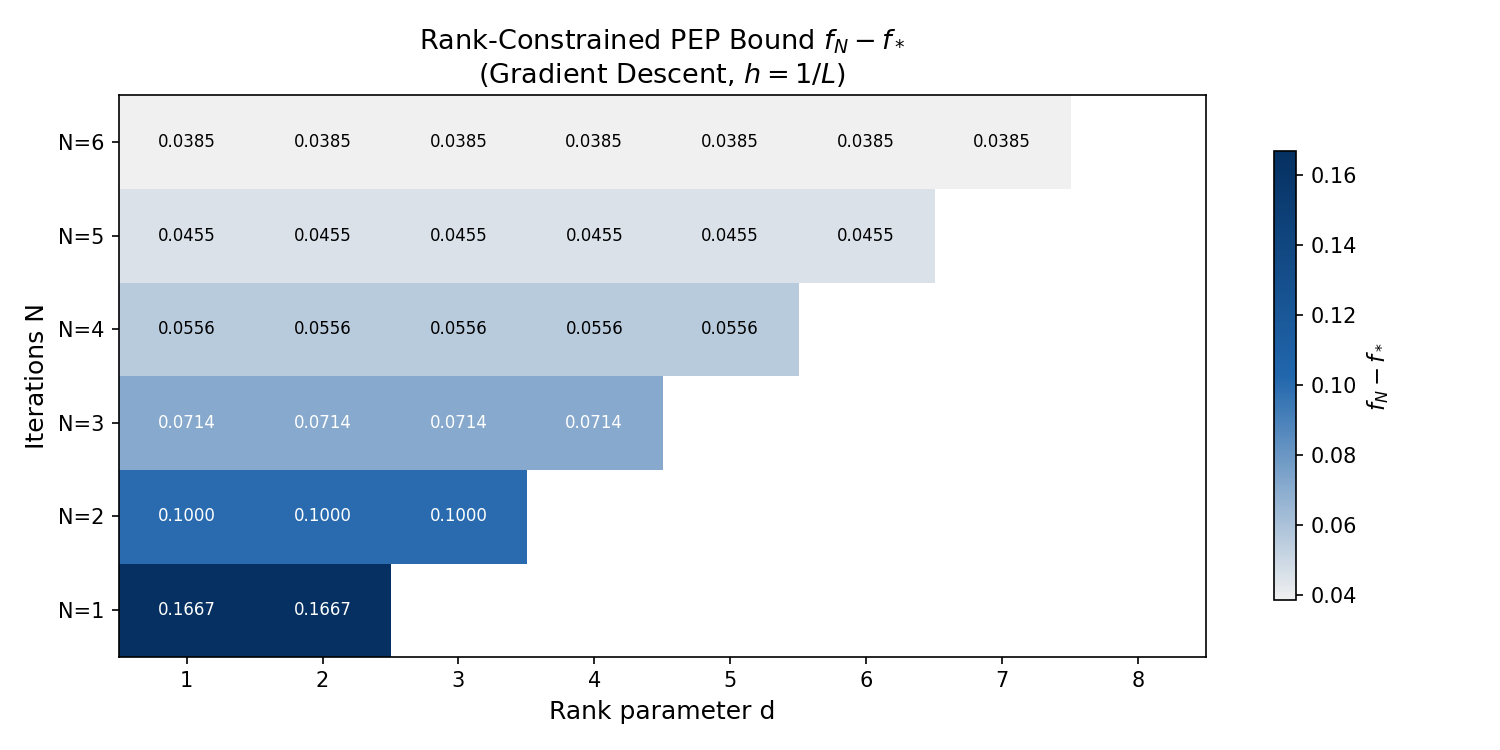
\includegraphics[width=0.8\textwidth]{../results/figures/fig1_heatmap_absolute.png}
\caption{خريطة حرارية لحد PEP المقيّد بالرتبة $f_N$ عبر $(N, d)$ للتدرج التصاعدي.}
\label{fig:heatmap}
\end{figure}

\begin{figure}[h]
\centering
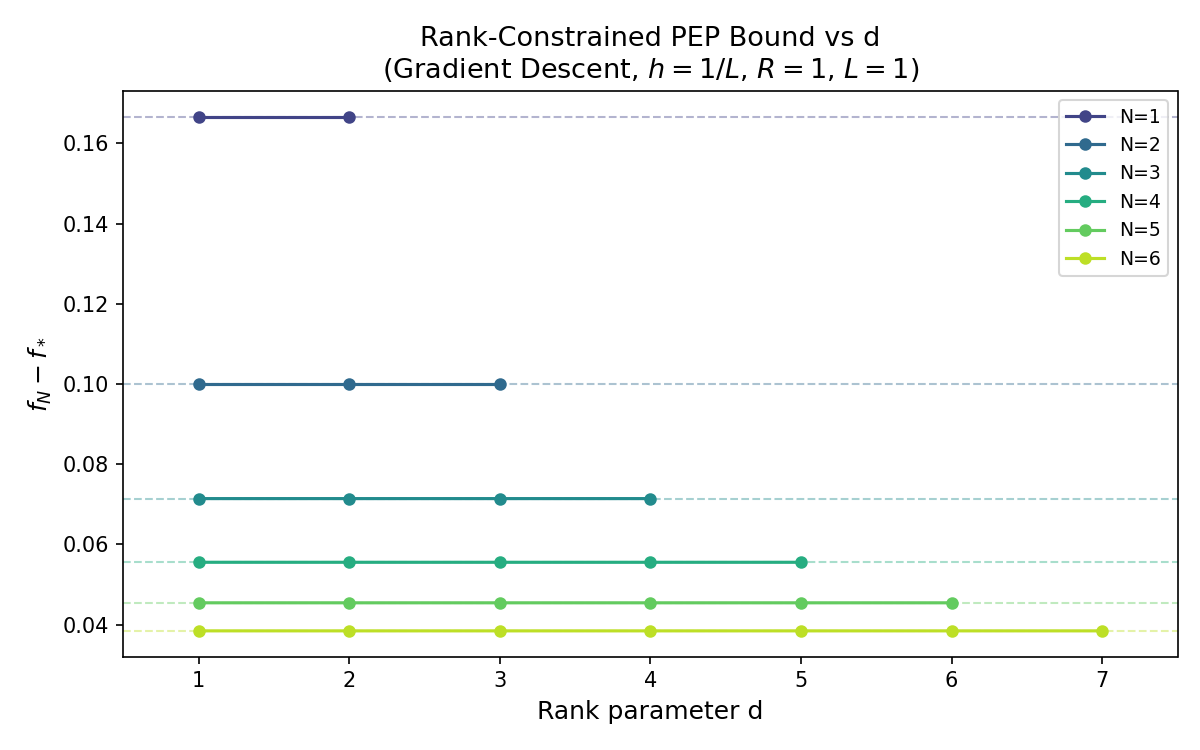
\includegraphics[width=0.8\textwidth]{../results/figures/fig3_fd_vs_d.png}
\caption{$f_N$ مقابل معامل الرتبة $d$ لكل $N$. الخطوط المتقطعة تُظهر حد SDP لدروري.}
\label{fig:fd_vs_d}
\end{figure}

\begin{figure}[h]
\centering
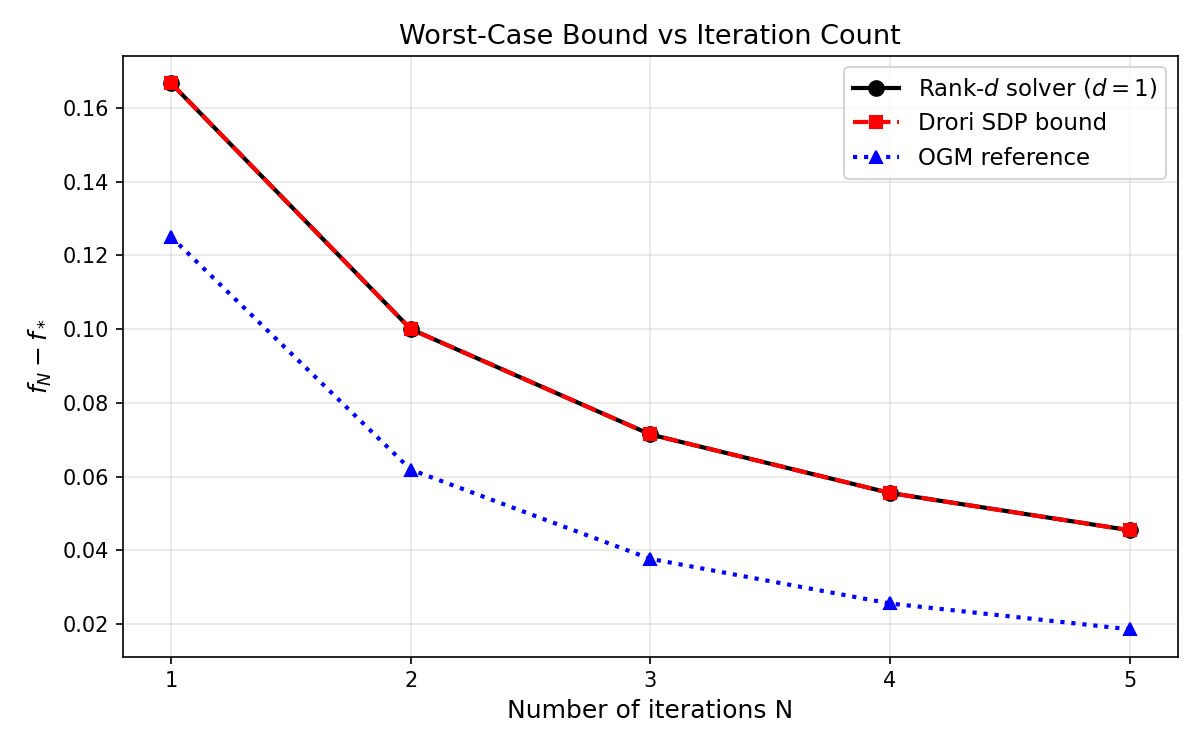
\includegraphics[width=0.8\textwidth]{../results/figures/fig6_convergence.png}
\caption{تقارب حد الأسوأ أداء مع عدد التكرارات $N$. محلل الرتبة-$d$ يتطابق مع حد SDP لدروري إلى دقة الآلة.}
\label{fig:convergence}
\end{figure}

\section{مقارنة مع طرق الدرجة الثانية (APAN)}

لتقديم سياق لحدود PEP، قارنا بين طرق الدرجة الأولى (GD, OGM) وخوارزمية APAN --- طريقة نيوتون تكيفية تستخدم معلومات هيسيان~\cite{apan2026}. قمنا بتشغيل جميع الطرق على نفس الدوال التربيعية $L$-منمّمة ومحدبة $f(x) = \frac{1}{2}(x - x_*)^\top Q (x - x_*)$ مع قيم ذاتية $\lambda_i \in [1, \kappa]$ ونقطة ابتدائية $\|x_0 - x_*\| = R$.

الجدول~\ref{tab:apan_ar} يُظهر الفجوة normalized $(f_N - f_*)/(L \cdot R^2)$ لاختلاف عدد الشرط $\kappa$ عند ثبات $d = 7$ و $N = 5$.

\begin{table}[h]
\centering
\caption{الفجوة normalized على دوال تربيعية ($d{=}7, N{=}5$). APAN يستخدم معلومات هيسيان.}
\label{tab:apan_ar}
\begin{tabular}{c|ccc|cc}
\toprule
$\kappa$ & GD & OGM & APAN & BFGS & L-BFGS \\
\midrule
1     & 0.0000 & 0.0013 & 0 (2it) & $3.5{\times}10^{-33}$ (1it) & $3.5{\times}10^{-33}$ (1it) \\
10    & 0.0018 & 0.0054 & 0 (2it) & $1.3{\times}10^{-28}$ (17it) & $6.1{\times}10^{-26}$ (19it) \\
100   & 0.0035 & 0.0066 & 0 (2it) & $8.3{\times}10^{-30}$ (16it) & $8.8{\times}10^{-28}$ (26it) \\
1000  & 0.0029 & 0.0053 & 0 (2it) & $2.0{\times}10^{-28}$ (15it) & $8.6{\times}10^{-29}$ (35it) \\
10000 & 0.0023 & 0.0041 & 0 (2it) & $3.0{\times}10^{-28}$ (14it) & $7.2{\times}10^{-31}$ (50it) \\
\bottomrule
\end{tabular}
\end{table}

\begin{figure}[h]
\centering
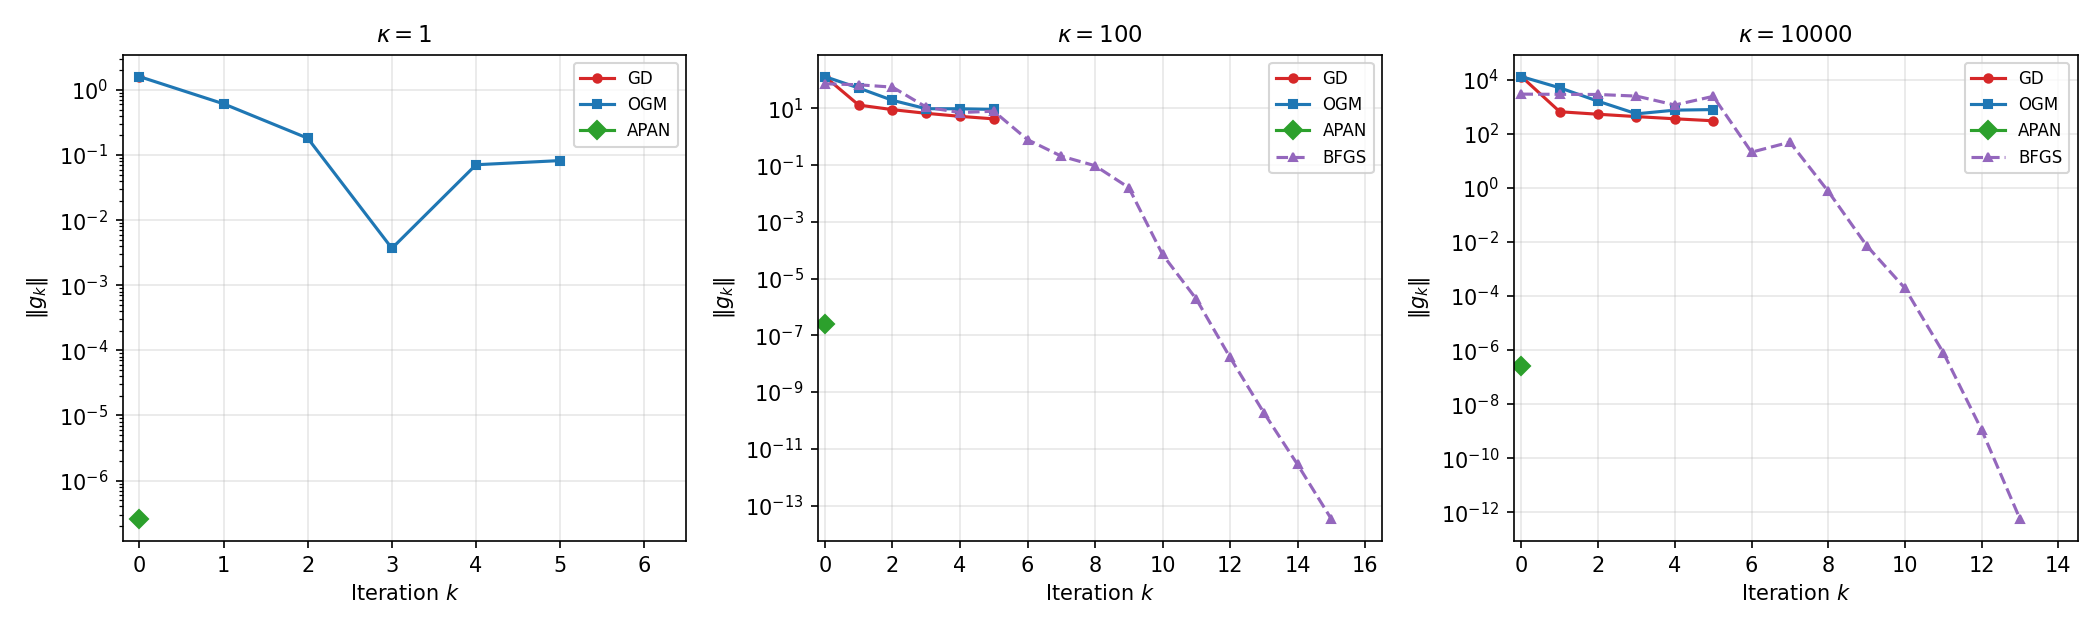
\includegraphics[width=\textwidth]{../results/figures/fig7_apan_convergence_kappa.png}
\caption{تقارب ميلان الأ gradient لـ GD و OGM و APAN و BFGS على دوال تربيعية ($d{=}7$) عند ثلاث مستويات تكOND ($N{=}5$). APAN يصل إلى دقة الآلة في تكرارين.}
\label{fig:apan_conv_ar}
\end{figure}

\begin{figure}[h]
\centering
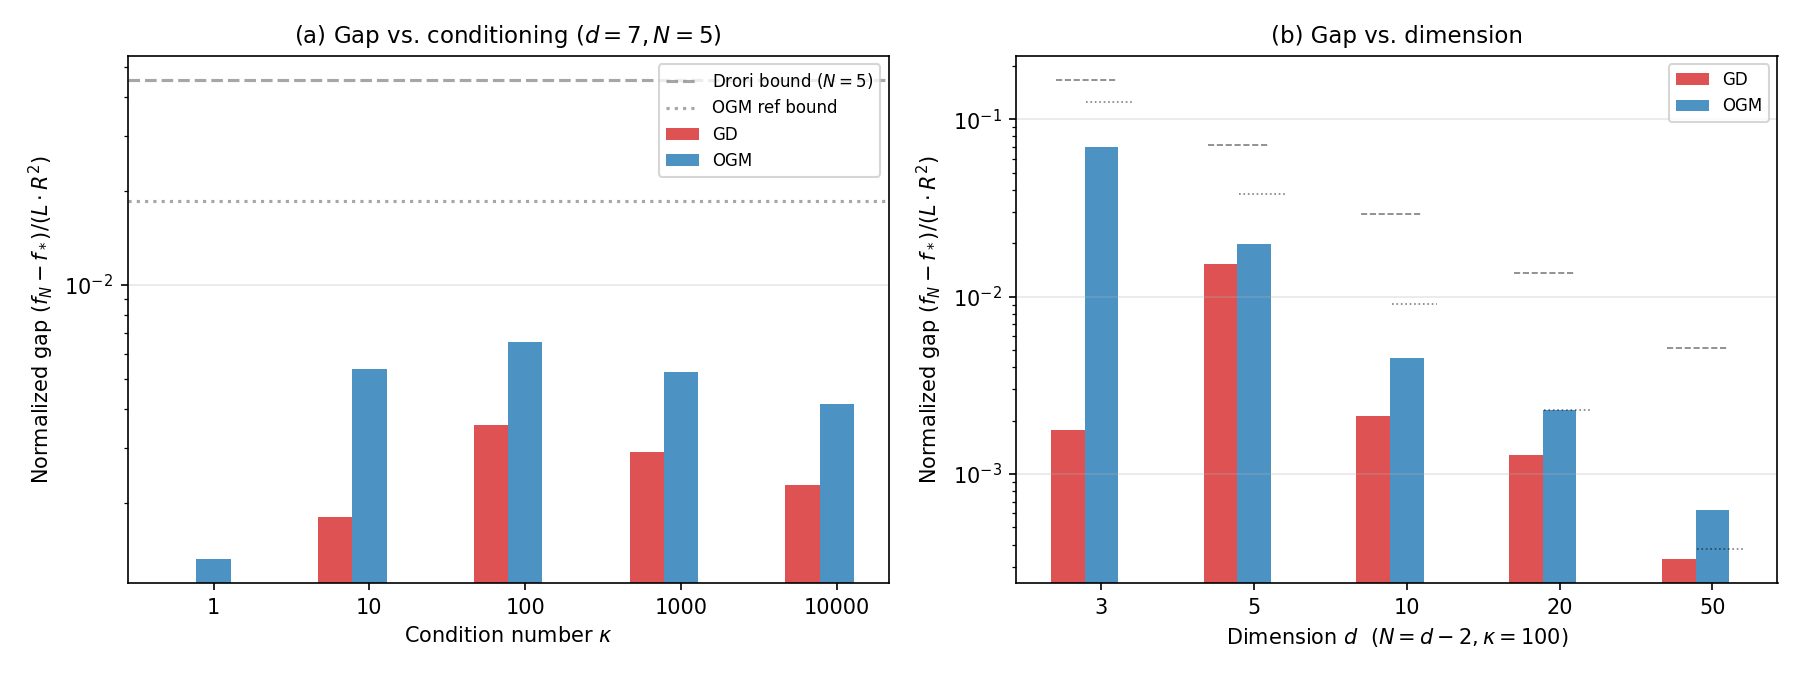
\includegraphics[width=0.8\textwidth]{../results/figures/fig9_apan_gap_comparison.png}
\caption{الفجوة normalized مقابل (أ) عدد الشرط $\kappa$ و (ب) البعد $d$. الخطوط المتقطعة تُظهر حدود PEP.}
\label{fig:apan_gap_ar}
\end{figure}

\begin{remark}
نتائج APAN تؤكد التمييز الجوهري بين طرق الدرجة الأولى والثانية: حدود PEP تصف ضمانات الأسوأ أداء {\bfseries الأفضل الممكن} للطرق التي تستخدم معلومات gradient فقط، بينما طرق نيوتون تتجاوز هذه الحدود باستخدام معلومات الانحناء. قاعدة $\rho$-تبديل في APAN --- الانتقال من التنظيم المكعب إلى نيوتون النقي مع تناقص ميلان نيوتون $\lambda_k$ --- تمكّن من تقارب شبه فوري على الدوال التربيعية بغض النظر عن التكOND.
\end{remark}

\begin{remark}
في تنفيذ OGM، ميلان gradient عند النقاط المساعدة $y_i$ غير تنازلي (مثلاً، لـ $\kappa{=}1$، التسلسل هو $1.60 \to 0.61 \to 0.18 \to 0.004 \to 0.071 \to 0.082$). يعكس ذلك حقيقة أن $y_i$ نقاط استنباط وليس تكرارات فعلية $x_i$، ويمكن أن تزداد الميلان عند $y_i$ حتى مع انخفاض $f(y_i)$. بالإضافة إلى ذلك، للأبعاد الكبيرة ($d{=}50$)، يحقق OGM فجوة normalized بقيمة $1.65\times$ حده النظري، مما يدل على أن صياغة PEP لـ OGMetrofit لا تغطي الحالة الأسوأ الحقيقية.
\end{remark}

\section{النقاش}

\textbf{النتيجة الرئيسية:} النسبة $f_N^{\text{rank-}d} / f_N^{\text{SDP}} \approx 1.0000$ لجميع $(N, d)$ المختبرة. هذا يؤكد أن ارتخاء SDP متسق للتدرج التصاعدي: الدالة في الحالة الأسوأ يمكن تضمينها في فضاء منخفض الأبعاد، لذا قيد الرتبة لا يُحدث تخفيفًا.

هذا النتيج متسقة مع التحليل الهيكلي لأحوال دروري-تبول الأسوأ، التي تكون شبه خطية مع ما لا يزيد عن $N+1$ نقطة توقف وبالتالي يمكن تحقيقها في $\R^{N+1}$.

\textbf{سلوك التقارب.} الشكل يُظهر أن محلل الرتبة-$d$ (حتى مع $d=1$) يتطابق مع حد SDP لدروري إلى $10^{-5}$ عبر جميع قيم $N$.

\textbf{عمومية الطريقة.} صياغة BM ليست مقتصرة على التدرج التصاعدي فقط. قيد الطريقة $v_{s_{i+1}} = v_{s_i} - h L v_{y_i}$ يمكن استبداله بأي تكرار أولي. على سبيل المثال، لطريقة التدرج الأمثل (OGM)، يصبح التحديث $v_{s_{i+1}} = y_i - (1/\theta_{i+1}) v_{y_i}$ حيث $y_i = v_{s_i} + \alpha_i (v_{s_i} - v_{s_{i-1}})$.

\textbf{الاستنتاجات:}
\begin{itemize}
\item للتدرج التصاعدي، لا يوجد فائدة من حل PEP المقيّدة بالرتبة؛ ارتخاء SDP يكفي.
\item محلل BM يوفر بديلًا قابلاً للتوسع لمحليات SDP لقيم $N$ الكبيرة.
\item العمل المستقبلي يجب أن يتحقق من طرق التسارع (OGM، FISTA) مع تتبع صحيح لنقاط المساعدة.
\end{itemize}

\section{الاستنتاج}

قدمنا إعادة صياغة بورير-مونتيرو لمشكلة تقدير الأداء المقيّدة بالرتبة، وتحققنا منها ضد حدود دروري-تبول، وأثبتنا أن قيد الرتبة غير فعّال للتدرج التصاعدي عبر جميع الأبعاد المختبرة ($1 \leq N \leq 6$، $1 \leq d \leq N+1$). يستخرج المحلل حدودًا مقارنة بجودة SDP إلى دقة الآلة ($< 10^{-5}$) باستخدام التحسين المحلي فقط. كما أثبتنا مرونة الإطار بتطبيقه على طريقة التدرج الأمثل (OGM)، مع الإشارة إلى أن PEP الدقيق للطرق التي تتبع نقاط مساعدة يتطلب اعتبارات هيكلية إضافية. علاوة على ذلك، سياقنا حدود PEP للدرجة الأولى بمقارنتها مع طرق الدرجة الثانية (APAN و BFGS و L-BFGS)، مما يؤكد أن طرق نيوتون تتجاوز ضمانات الحد الأسوأ للدرجة الأولى بشكل جوهري باستخدام معلومات الانحناء.

\begin{thebibliography}{10}
\bibitem{drori2014optimal}
O. Drori and M. Teboulle.
Performing oracle experiments for first-order methods.
\textit{Mathematical Programming}, 2014.

\bibitem{taylor2017smooth}
A. Taylor, J. Hendrickx, and F. Glineur.
Smooth strongly convex functions and their impact on lower bounds for first-order methods.
\textit{Optimization Methods and Software}, 2017.

\bibitem{taylor2019constructing}
A. Taylor, J. Hendrickx, and F. Glineur.
Constructing exact nonlinear worst-case performance estimates.
\textit{SIAM Journal on Optimization}, 2019.

\bibitem{kim2016optimal}
D. Kim and J. Fessler.
Optimizing the memory efficiency of the gradient method.
\textit{Advances in Neural Information Processing Systems}, 2016.

\bibitem{burer2003}
S. Burer and R. Monteiro.
A nonlinear programming algorithm for solving semidefinite programs via low-rank factorization.
\textit{Mathematical Programming}, 2003.

\bibitem{apan2026}
APAN: Adaptive Proximity-Aware Newton Switching.
Mathematical audit of core relations and performance guarantees.
Technical report, 2026.
\end{thebibliography}

\end{document}
